\documentclass{ltjbook}
\usepackage{docmute} 
\usepackage{../../myStyle} 

\begin{document}
% \chapter{Rによるベイズ推定}
\chapter{Bayesian Estimation using R}
\label{m29_brms}
% JASPによる分析は比較的簡単で，わかりやすかったのではないでしょうか。とはいえ，それはユーザーインターフェイスのおかげかもしれませんね。すなわちクリック，タップ，ドロップなどで視覚的に操作できるGUIのおかげで，簡単便利とおもえるわけです。
The analysis using JASP is relatively simple and understandable, don't you think? However, that might be thanks to the user interface. That is, thanks to the GUI, which you can visually operate with clicks, taps, and drops, it seems easy and convenient.
% もちろんそれを否定するわけではありませんが，GUIの欠点として，やったことを他人と共有する難しさがあります。「これをこうして・・・」と動きを言葉で説明するのは難しいことです。共有できないことは再現できないことにつながりますし，ひどい場合は「機械が勝手にやったので，自分では何をやったかわかりません」ということにもなりかねません\footnote{実際，GUIの統計ソフトウェアで指導していると困るのがここで，自分では気づかない，デフォルトで設定されている条件でぶんせきしているとか，自分がどういう動きをしたかがわからないので，統計の原理や仮定を違えておかしな分析を無自覚にやっている，ということにもなります。}。その点，RなどCUIで実行指令書を残しておくやり方は，一見面倒なように思えるのですが，記録が残ることと再現可能性の高さから，研究教育の面では向いています。
Of course, I'm not denying that, but one drawback of GUI is the difficulty in sharing what you've done with others. It's hard to explain movements in words like "do this and then that..." If you can't share something, it leads to a lack of reproducibility and in the worst cases, it can come down to "the machine did it on its own, I don't know what I did" \footnote{Indeed, one of the challenges in teaching with GUI statistical software is that students might not realize that they are analyzing conditions set by default, or they don't know what actions they took, which could lead to an unconscious violation of statistical principles and assumptions.}. In this respect, the method of leaving execution instructions in R and other CUI may seem cumbersome at first, but the recordability and high reproducibility make it suitable for research and education.

% さて，Rでベイズ推定できるのかと言えば，当然それは可能です。今回はその方法について，演習的にやっていきましょう。と言っても，ベイズ対応のパッケージを使うだけなのですが。
Well, when it comes to whether it's possible to perform Bayesian estimation in R, of course it is. This time, let's go through the process in a practical manner. Even though all we are doing is using a Bayesian-friendly package.
% 簡単なモデルであれば確率分布の計算から解析的に答えを出すことはできますが，今後のことも考えてMCMC法による方法を説明します。これはRの\texttt{brms}パッケージ\citep{brmsCite1,brmsCite2}で提供されています。
Even with a simple model, it is possible to derive results analytically from the calculation of probability distribution, but considering the future, I will explain the method by MCMC. This is provided in the R package brms.
% Rパッケージの\texttt{brms}を使うと，一般線形モデルが簡単に実装できます。関数名が\texttt{lm}から\texttt{brm}に変わるだけで，MCMCをつかった線形モデルのベイズ推定を行うことができ，またその結果の可視化も簡単に行えます。\texttt{lm}関数と同じく，説明変数を離散型(factor型)にしておくと，要因の効果の大きさが推定でき，\texttt{brms}パッケージの\verb|conditional_effects|関数を使うと要因ごとに周辺化された結果も図示されます。
Using the R package \texttt{brms}, you can easily implement general linear models. Simply by changing the function name from \texttt{lm} to \texttt{brm}, you can perform Bayesian estimation of linear models using MCMC, and it's also easy to visualize the results. Like the \texttt{lm} function, if you set the explanatory variables to discrete (factor-type), the effect size of the factor can be estimated, and by using the \verb|conditional_effects| function of the \texttt{brms} package, the marginalized results for each factor are also shown in the graph.
% \section{環境の準備}
\section{Preparing the Environment}
% まずは環境の準備です。いつもの通り，次の3つのステップを経てください。
First, we need to prepare the environment. As always, please follow these three steps.
% \paragraph{RStudioの起動}RStudioを起動してください。パッケージのインストールをするときなど，管理人権限が必要になるケースがあります。
\paragraph{Starting RStudio} Please start RStudio. There are cases when administrator rights are required, such as when installing packages.
% \paragraph{プロジェクトを開く}プロジェクトは前回作成した物で良いと思います。同じフォルダの中で，スクリプトファイルだけ変えれば良いでしょう。メニューからプロジェクトを開き(FIle$\to$Open Project)，RStudioの右上などで，プロジェクトが開いていることを確認しましょう($\to$図\ref{fig::20_01})。
\paragraph{Open the project} You can use the project that you created last time. Within the same folder, you only need to change the script file. Open the project from the menu (File$\to$Open Project), and confirm that the project is open in the upper right corner of RStudio ($\to$Figure \ref{fig::20_01}).
% \paragraph{Rスクリプトを開く}今日のコードを書くためのRスクリプトファイルを準備します。File > NewFile > R Scriptと進み，何も書いてないRスクリプトの画面を表示させてください。真っ白いファイルが開いたら問題ありません。
\paragraph{Open the R script} Prepare an R script file to write today's code. Please proceed with File > NewFile > R Script and display the screen of the R script without writing anything. If a completely white file is open, there is no problem.

% 続いて，ベイズ推定用のパッケージを準備します。\texttt{brms}パッケージ\footnote{ベイズで(Bayesian),回帰モデルを(Regression Mode)実行する，Stanを使ってね(using Stan)，という意味です。Stanとは\keyterm{確率的プログラミング言語}{かくりつてきぷろぐらみんぐげんご}{stocastic programming language}の一種で，要するに乱数発生器を作ってくれるソフトウェアのことです。}をインストールするのですが，このパッケージをインストールする\textbf{前に}，このパッケージが必要とするコンパイラを用意する必要があります。
Next, we will prepare a package for Bayesian estimation. The \texttt{brms} package\footnote{It means to perform Bayesian, regression model, using Stan. Stan is a type of probabilistic programming language, essentially a software that generates random numbers.} is installed, but \textbf{before} installing this package, you need to prepare the compiler that this package requires.
% 詳しくは \url{https://github.com/stan-dev/rstan/wiki/RStan-Getting-Started-(Japanese)}のサイトに説明がありますが\footnote{「RStan Getting Started (Japanese)」でググると出てきます。}\footnote{\citet{Baba201907}にも導入についての詳しい説明があります。}，Windowsユーザの場合はまず，\texttt{code:\ref{code:27_01}}を実行してください。
There are detailed explanations on the \url{https://github.com/stan-dev/rstan/wiki/RStan-Getting-Started-(Japanese)} site\footnote{It will appear if you Google "RStan Getting Started (Japanese)".}\footnote{There is also a detailed introduction in \citet{Baba201907}.}, but if you are a Windows user, first, please execute \texttt{code:\ref{code:27_01}}.
\begin{lstlisting}[language=c++,label={code:27_01},caption={Installing necessary tools}]
pkgbuild::has_build_tools(debug = TRUE)
\end{lstlisting}


% コンパイラであるRtoolsが環境にない場合には，ポップアップウィンドウが出てきてRtoolsをインストールするか聞いてくるでしょう。Yesをクリックして1分ぐらいインストールが終わるのを待って下さい。
If the compiler Rtools isn't in your environment, a pop-up window will appear asking if you want to install Rtools. Please click on "Yes" and wait for about a minute for the installation to complete.

% Macユーザの場合は，\url{https://github.com/rmacoslib/r-macos-rtools}にいき，Release page から\texttt{macos-rtools-4.0.0.pkg}を選択してインストールします\footnote{2020年11月28日段階での状況です。}。
For Mac users, go to \url{https://github.com/rmacoslib/r-macos-rtools}, select \texttt{macos-rtools-4.0.0.pkg} from the Release page and install it\footnote{This is the situation as of November 28, 2020.}.
% OSがCatalinaであれば，さらに
% \begin{lstlisting}[language=c++,label={code:27_01},caption={オブジェクトに代入}]
% install.packages("Rcpp", repos = "https://rcppcore.github.io/drat")
% \end{lstlisting}
% とする必要があります。

% これで準備OKで，これではじめて\texttt{brms}パッケージをインストールできるようになりました\footnote{この環境構築は初心者にはとっても荷が重いところですね。困ったらいつでも連絡してきてください。どうしても難しい場合は，サーバが利用できますのでこれまた連絡してください。}。
You are now ready to install the brms package with this. This environment setup is very heavy for beginners. Please feel free to contact me if you have any trouble. If it really becomes too difficult, you can use a server, so please do not hesitate to contact me for this as well.
% 関連する複数のパッケージを次々取り込んで行きますので，少し時間がかかるかもしれません。
It might take some time as we will be incorporating multiple related packages one after another.
% RStudioのパッケージのところから\texttt{brms}を入力してインストール，あるいはRのスクリプトとして\texttt{code:\ref{code:27_02}}のようにすればインストールが始まります。
Enter \texttt{brms} in the package section of RStudio to install, or start installing it by typing as \texttt{code:\ref{code:27_02}} in the R script.


\begin{lstlisting}[language=c++,label={code:27_02},caption={Install a package}]
install.packages("brms")
\end{lstlisting}


% この作業は環境整備なので一度だけでよく，無事にインストールできれば今後はパッケージを呼び出すだけでよくなります。
This task is setup, so it only needs to be done once. If you can install it successfully, you will just need to call the package from then on.
% \section{回帰分析の推定}
\section{Estimation of Regression Analysis}
% それでは回帰分析の推定をしていきましょう。使うデータは第\ref{m09_Regression}講で使った高校・大学の成績についてのものです。復習がてら，\texttt{code:\ref{code:27_03}}実行しましょう。
Let's proceed with the estimation of regression analysis. The data we will use is about high school and university grades, which we used in Lecture \ref{m09_Regression}. As a review, let's execute \texttt{code:\ref{code:27_03}}.
\begin{lstlisting}[language=c++,label={code:27_03},caption={回帰分析をやってみる}]
# データを入力
koukou <- c(2.13,2.42,2.26,3.87,3.90,2.43,3.44,
2.15,2.18,3.00,3.42,2.55,3.19,3.05,2.52)
daigaku <- c(460,500,473,620,690,512,582,
550,485,650,593,528,585,569,518)
# データフレーム型に組み上げる
seiseki <- data.frame(koukou,daigaku)

# データは図にする
ggplot(seiseki,aes(x = koukou, y = daigaku)) +
    geom_point() +
    geom_smooth(method = "lm", se = F)

# 線形モデルはlm関数。従属変数~説明変数の形で書く
fit <- lm(daigaku ~ koukou, data = seiseki)
# 結果をわかりやすく表示
summary(fit)
\end{lstlisting}


% \paragraph{コード解説}
\paragraph{Code Explanation}
\begin{description}
   \item[2-3 lines] Inputting data from high school and university years.
   \item[5th line] Constructing each data into a data frame format.
   \item[8-10 lines] Drawing using ggplot.
   \item[13th line] Conducting a regression analysis.
   \item[15th line] Outputting the results.
\end{description}


% これの結果は次のようなものでした(\texttt{Rの出力\ref{RS:out27_01}})。
The result of this was as follows (R's output \ref{RS:out27_01}).
\begin{Rscreen}{lm output}{out27_01}
   \begin{verbatim}
> summary(fit)

Call:
lm(formula = daigaku ~ koukou, data = seiseki)

Residuals:
    Min      1Q  Median      3Q     Max 
-31.425 -21.896  -6.906  -1.207  80.110 

Coefficients:
            Estimate Std. Error t value Pr(>|t|)    
(Intercept)   288.74      43.00   6.715 1.44e-05 ***
koukou         93.72      14.85   6.313 2.69e-05 ***
---
Signif. codes:  0 ‘***’ 0.001 ‘**’ 0.01 ‘*’ 0.05 ‘.’ 0.1 ‘ ’ 1

Residual standard error: 34.36 on 13 degrees of freedom
Multiple R-squared:  0.754,	Adjusted R-squared:  0.7351 
F-statistic: 39.85 on 1 and 13 DF,  p-value: 2.688e-05
\end{verbatim}
\end{Rscreen}

% 回帰係数は切片が288.74，傾きが93.72と推定され，それらが0ではないと帰無仮説に対する検定結果が示されています。またモデル全体の適合について，$F(1,13)=39.85,p=0.000002688$という結果や，$R^2=0.754$などが示されています\footnote{少し補足。$p$値は$2.688\times 10^{-5}$という意味です。桁数の表示が長くなりすぎるので，機械はこのような省略記号を書きます。また適合度を表す$R^2$の値ですが，ここではMultiple R-squaredの値をそのまま書いています。この値はサンプルサイズによって過大評価されることがあるので，論文などではそれを補正した「自由度調節済み$R^2$」が使われることもあります。}
The estimated regression coefficient is 288.74 for the intercept and 93.72 for the slope, indicating that they are not zero against the null hypothesis. For the overall fit of the model, results such as $F(1,13)=39.85, p=0.000002688$ and $R^2=0.754$ are indicated\footnote{A little supplement. The value of $p$ means $2.688\times 10^{-5}$. Machines write such abbreviations so that the number of digits does not become too long. Also, about the value of $R^2$ representing the fit, here we are simply writing the value of Multiple R-squared. This value can be overrated depending on the sample size, so in papers and so on, the "adjusted $R^2$ " that corrects it is often used.}

% 早速これをベイズ推定していきましょう。何がどう変わるのでしょうか。
Let's go ahead and do the Bayesian estimation right away. I wonder what will change and how?
% まずはパッケージ\texttt{brms}を読み込み，回帰分析の関数を\texttt{lm}から\texttt{brm}に変えるだけでオッケーです(\texttt{code:\ref{code:27_04}})。
First, load the brms package, and you're good to go just by changing the regression analysis function from lm to brm (code:\ref{code:27_04}).

\begin{lstlisting}[language=c++,label={code:27_04},caption={ベイズ推定してみる}]
library(brms)
fit.brm <- brm(daigaku ~ koukou, data = seiseki)
print(fit.brm)
\end{lstlisting}


% 画面にさまざまなメッセージが出力されたかと思いますがそれは後で説明するとして，とりあえず最後の3行目を実行して示された回帰分析の結果を確認してみましょう。
Various messages might have appeared on your screen, but we will explain those later. For now, let's check the results of the regression analysis that was executed and displayed in the last three lines.

% 一行目に\texttt{Family: gaussian }とあります。これは正規分布(gaussian curve)を使ったモデルであることが示されています。2，3行目にモデルの説明，4行目にデータの説明があった後，6行目には\texttt{Samples:}とあります。これはデータ，標本のことを指しているのではなく，MCMC法によって得られた乱数のサンプルのことを意味しています。MCMCの表記等については後でまとめて説明します。
The first line says \texttt{Family: gaussian}. This indicates that it is a model that uses a normal distribution (gaussian curve). After the model's explanation in lines 2 and 3, and the data's explanation in line 4, line 6 says \texttt{Samples:}. This is not referring to the data or samples, but refers to the samples of random numbers obtained by the MCMC method. The notation of MCMC and others will be explained later.

% また，MCMCによる結果は毎回乱数を発生させて計算させています。ここに示した結果は私の環境での結果であって，皆さんがやってみると少し違った数字が出てくるかもしれません。というのも，パソコンがかわると生成される擬似乱数も変わってしまうからです。MCMC法はあくまでも近似計算ですから，厳密に一致するかどうかを考えるのではなく，だいたいあっているかどうかで判断してください\footnote{そんな適当でいいのか！と思うかもしれません。でも乱数を大量に発生させると，ほとんど同じ結果になります。また生成する乱数の数を10倍にすると，一桁精度がアップします。それでも完璧に一緒，というわけにはいきませんが，そんな場合は擬似乱数の開始点\texttt{seed}を固定することで，再現可能な乱数を得ることができます。}。
Also, the results from MCMC are calculated by generating random numbers each time. The results shown here are from my environment, so you might get slightly different numbers if you try it out. This is because the pseudorandom numbers generated will change when the computer changes. Since the MCMC method is an approximation, don't think about whether it matches exactly, but judge whether it's roughly correct or not\footnote{You might think if it's okay to be that arbitrary! But when a large amount of random numbers is generated, the results become almost the same. If you increase the number of generated random numbers tenfold, you increase the precision by one digit. It is not exactly the same, but in such cases, by fixing the starting point of pseudorandom numbers, the \texttt{seed}, it is possible to get reproducible random numbers.}.

% 係数などは\texttt{Population-Level Effects }というところに書かれているもので，切片(Intercept)の推定値(Estimate)が288.37，説明変数である高校の成績にかかる傾きが93.86であることが示されています。続いて標準誤差，95\%確信区間の下限(lower)(\texttt{l-95\%CI})，上限(upper)(\texttt{u-95\% CI})が示されています。検定ではなく，95\%区間を見てそれが0を跨いでいるかどうかで，検定と同じような判断ができるということですね。
These values such as coefficients are written under "Population-Level Effects". Intercept estimate is 288.37 which indicates that the slope of the high school grades, an explanatory variable, is 93.86. Following, standard error, lower limit of the 95% confidence interval (\texttt{l-95\%CI}), and upper limit (\texttt{u-95\% CI}) are indicated. The judgment similar to a test can be made not from a test but from checking whether the 95% interval overlaps zero.

% 最後にもう1つの推定値，$\sigma$が\texttt{Family Specific Parameters}のところに現れています\footnote{線形回帰は$Y_i \sim N(\beta_0 + \beta_1 X_i , \sigma)$で，未知数は$\beta_0,\beta_1,\sigma$の3つであったことを思い出してください。}。
Finally, another estimated value, $\sigma$, appears in the \texttt{Family Specific Parameters} section\footnote{Remember that in linear regression, $Y_i \sim N(\beta_0 + \beta_1 X_i , \sigma)$, where the unknowns were three: $\beta_0,\beta_1,\sigma$.}.

% \texttt{Rの出力\ref{RS:out27_02}}が基本的な結果の情報です。\texttt{lm}関数を使った最尤推定の結果とほとんど同じ数字になっていることがわかります。結果はそれほど変わらないのですが，推定値が分布として得られていることが大きく異なる点です。
The output of R\ref{RS:out27_02} is the basic information of the results. You will find that the numbers are almost the same as the results of the maximum likelihood estimation using the \texttt{lm} function. While the results don't change much, the major difference is that the estimates are obtained as a distribution.
daigaku: university
koukou: high school
seiseki: grades/marks

% このことをわかりやすく表示するために，\texttt{plot(fit.brm)}としてみましょう。図\ref{fig::29_01}のように，分析結果がプロットされます。
To display this in an easy-to-understand way, let's try \texttt{plot(fit.brm)}. As shown in Figure \ref{fig::29_01}, the analysis results are plotted.
\begin{figure}[ht]
	\centering
	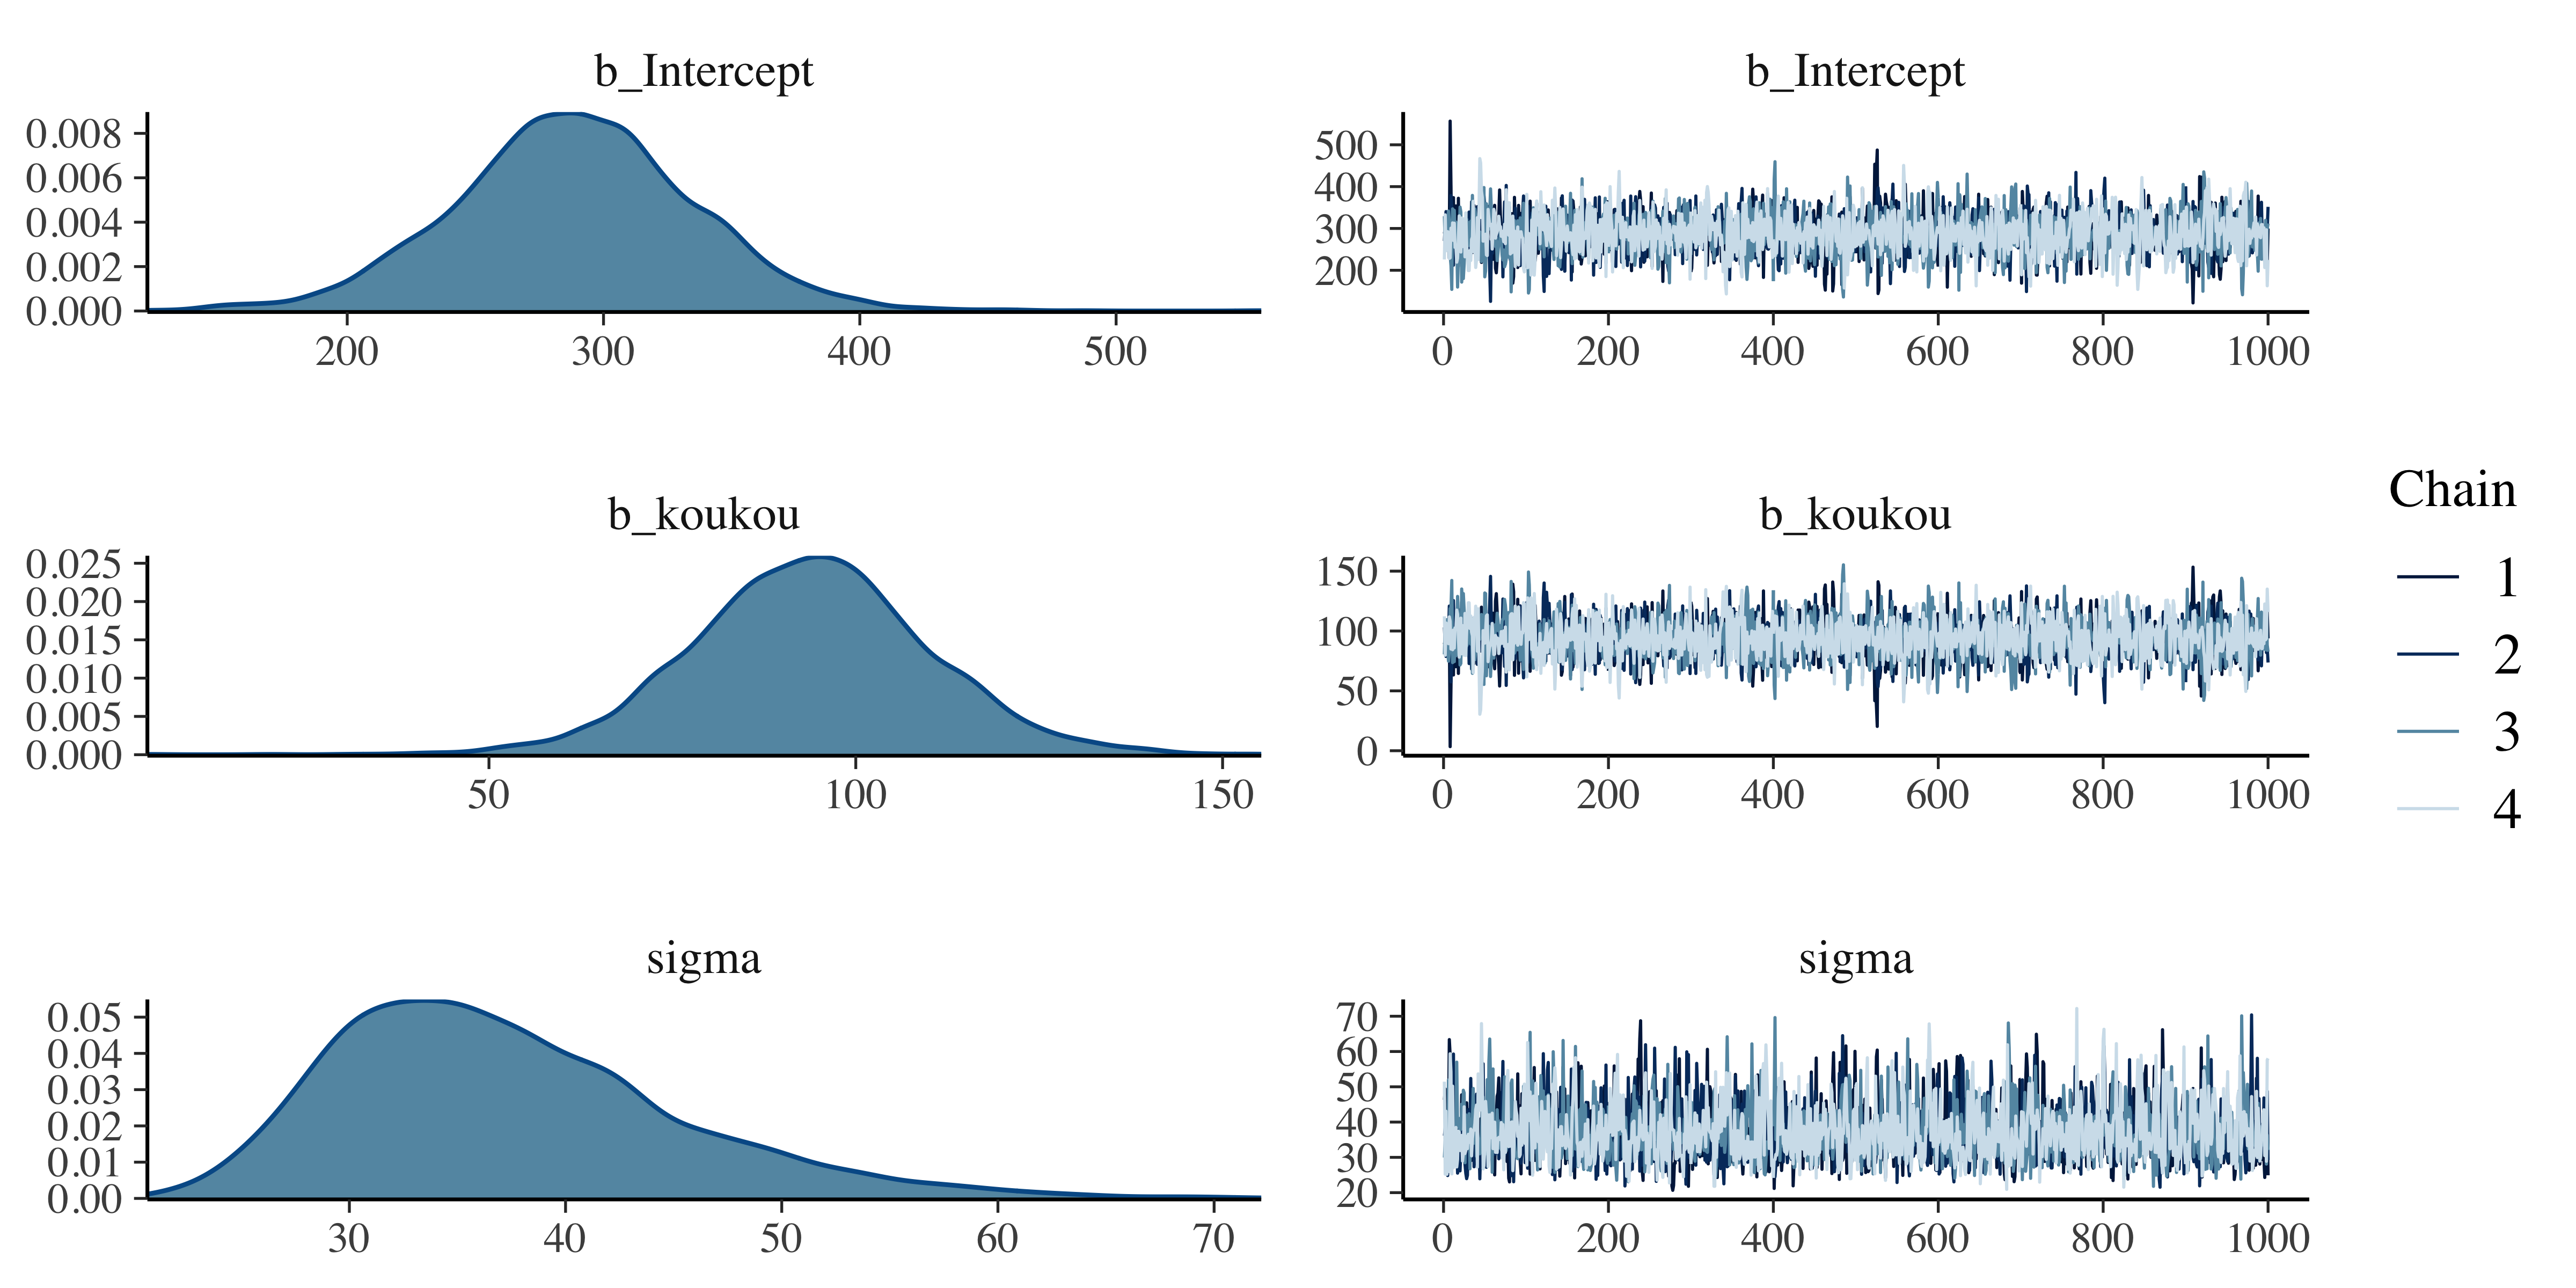
\includegraphics[keepaspectratio,width=0.8\linewidth]{../images/27_bayesian3/Rplot27_01.png}
	\caption{ベイズ法による回帰係数の推定}
	\label{fig::29_01}
\end{figure}

% この図の左側にあるのが，事後分布の形です。推定値である288.37や93.86は分布の平均値(\keytermL{EAP推定値}{EAPすいていち})で，この分布のピーク(MAP推定値)ではないことに注意してください。MAP推定値が欲しい場合は，別途\texttt{bayestestR}パッケージ\citep{bayestestR}を導入し，\verb|map_estimate|関数を実行する必要があります(\texttt{code:\ref{code:27_05}})。
The shape on the left side of this diagram is that of the posterior distribution. The estimates 288.37 and 93.86 are mean values of the distribution (EAP estimates), not the peak of the distribution (MAP estimates). Please note this. If you want the MAP estimates, you need to separately install the `bayestestR` package and run the \verb|map_estimate| function (See code:\ref{code:27_05}).

\begin{lstlisting}[language=c++,label={code:27_05},caption={結果の表示}]
install.packages(bayestestR)
library(bayestestR)
map_estimate(fit.brm)
\end{lstlisting}

% \paragraph{コード解説}
\paragraph{Code explanation}
\begin{description}
   \item[1行目] If you don't have the \texttt{bayestestR} package, you can install it with this line.
   \item[2行目] Load the package.
   \item[3行目] Feed the analysis result into the \verb|map_estimate| function.
\end{description}


% 最小二乗法や最尤法と違って，結果が分布で表されるという感覚が掴めてきたでしょうか。続いてはこの分布が乱数によって生成されていることに注目してみたいと思います。
Unlike the least squares method and the maximum likelihood method, have you been able to grasp the concept that the result is represented by a distribution? Next, I would like to focus on the fact that this distribution is generated by random numbers.
% \subsection{MCMC法の評価}
\subsection{Evaluation of MCMC Method}
% 既に述べたように，MCMCは乱数発生法であり，事後分布からのサンプリングでもって結果のヒストグラムを描くのでした。ヒストグラムが確率分布の稜線を描いてくれるからです。ただし，乱数ですから毎回違う結果が出ます。乱数がちゃんと事後分布からのものであるかどうかも，チェックしなければなりません。それらの情報について書いてあるのが，結果の6行目のあたりにあるのです(\texttt{Rの出力\ref{RS:out27_03}})。これを読み解いていきましょう。
As we have already mentioned, MCMC is a random number generation method, and its results are generated by sampling from the posterior distribution to draw a histogram. This is because the histogram will draw the ridgelines of the probability distribution. However, since it is based on random numbers, the results will vary each time. Also, we must check whether the random numbers properly originate from the posterior distribution. Information about this can be found around the sixth line of the result (\texttt{R's output \ref{RS:out27_03}}). Let's interpret this.

\begin{Rscreen}{MCMCの評価}{out27_03}
   \begin{verbatim}
Samples: 4 chains, each with iter = 2000; warmup = 1000; thin = 1;
    total post-warmup samples = 4000
\end{verbatim}
\end{Rscreen}


% MCMC法はステップ・バイ・ステップで，一歩ずつ次の乱数を生み出していってます。このMCMCサンプルは，推定したいパラメータの代表候補たちです。内部に保存されているデータを抜き出したのが図\ref{fig::27_02}です。今回は切片(\verb|b_intercept|)と傾き(\texttt{b})と誤差の散らばり度(\texttt{sigma})について，毎回のステップで得られた乱数の値が書かれています。たとえば傾きは$77.55104 \to 100.42599 \to 133.46551 \to 77.90979 \to \cdots$というように，前回の値を軸にしながら次々と乱数を生み出していってるのです。正確には，ここには3つの変数があり，赤枠で囲んでいるようにこの3つの変数からなる同時確率空間からサンプリングしてきます。つまり$(336.0793,77.55104,32.49790)\to (283.5139,100.42599,41.52797) \to \cdots$というように，3つずつセットでステップを踏んでいることになります。これがどんどん積み重なっていく，ステップの様子を示したのが図の中頃にあるギザギザの折れ線であり，これをまとめ上げて積み重ねたヒストグラムが最後に事後分布として得られる，というのが基本原理です。
The MCMC method generates a sequence of random numbers step by step. These MCMC samples are representative candidates of the parameters you want to estimate. Figure \ref{fig::27_02} presents the data stored internally. This time, the random numbers obtained at each step are recorded for the intercept (\verb|b_intercept|), slope (\texttt{b}), and degree of error scatter (\texttt{sigma}). For example, the slope generates random numbers one after another, like $77.55104 \to 100.42599 \to 133.46551 \to 77.90979 \to \cdots$, with the previous value as the axis. Precisely, there are three variables here, and we are sampling from the joint probability space of these three variables, as enclosed in the red frame. In other words, we are stepping in sets of three, such as $(336.0793,77.55104,32.49790)\to (283.5139,100.42599,41.52797) \to \cdots$. The zigzag broken line in the middle of the figure shows the buildup of these steps, and gathering these creates the stacked histogram, which finally produces the posterior distribution as per the basic principle.

\begin{figure}[ht]
   \centering
   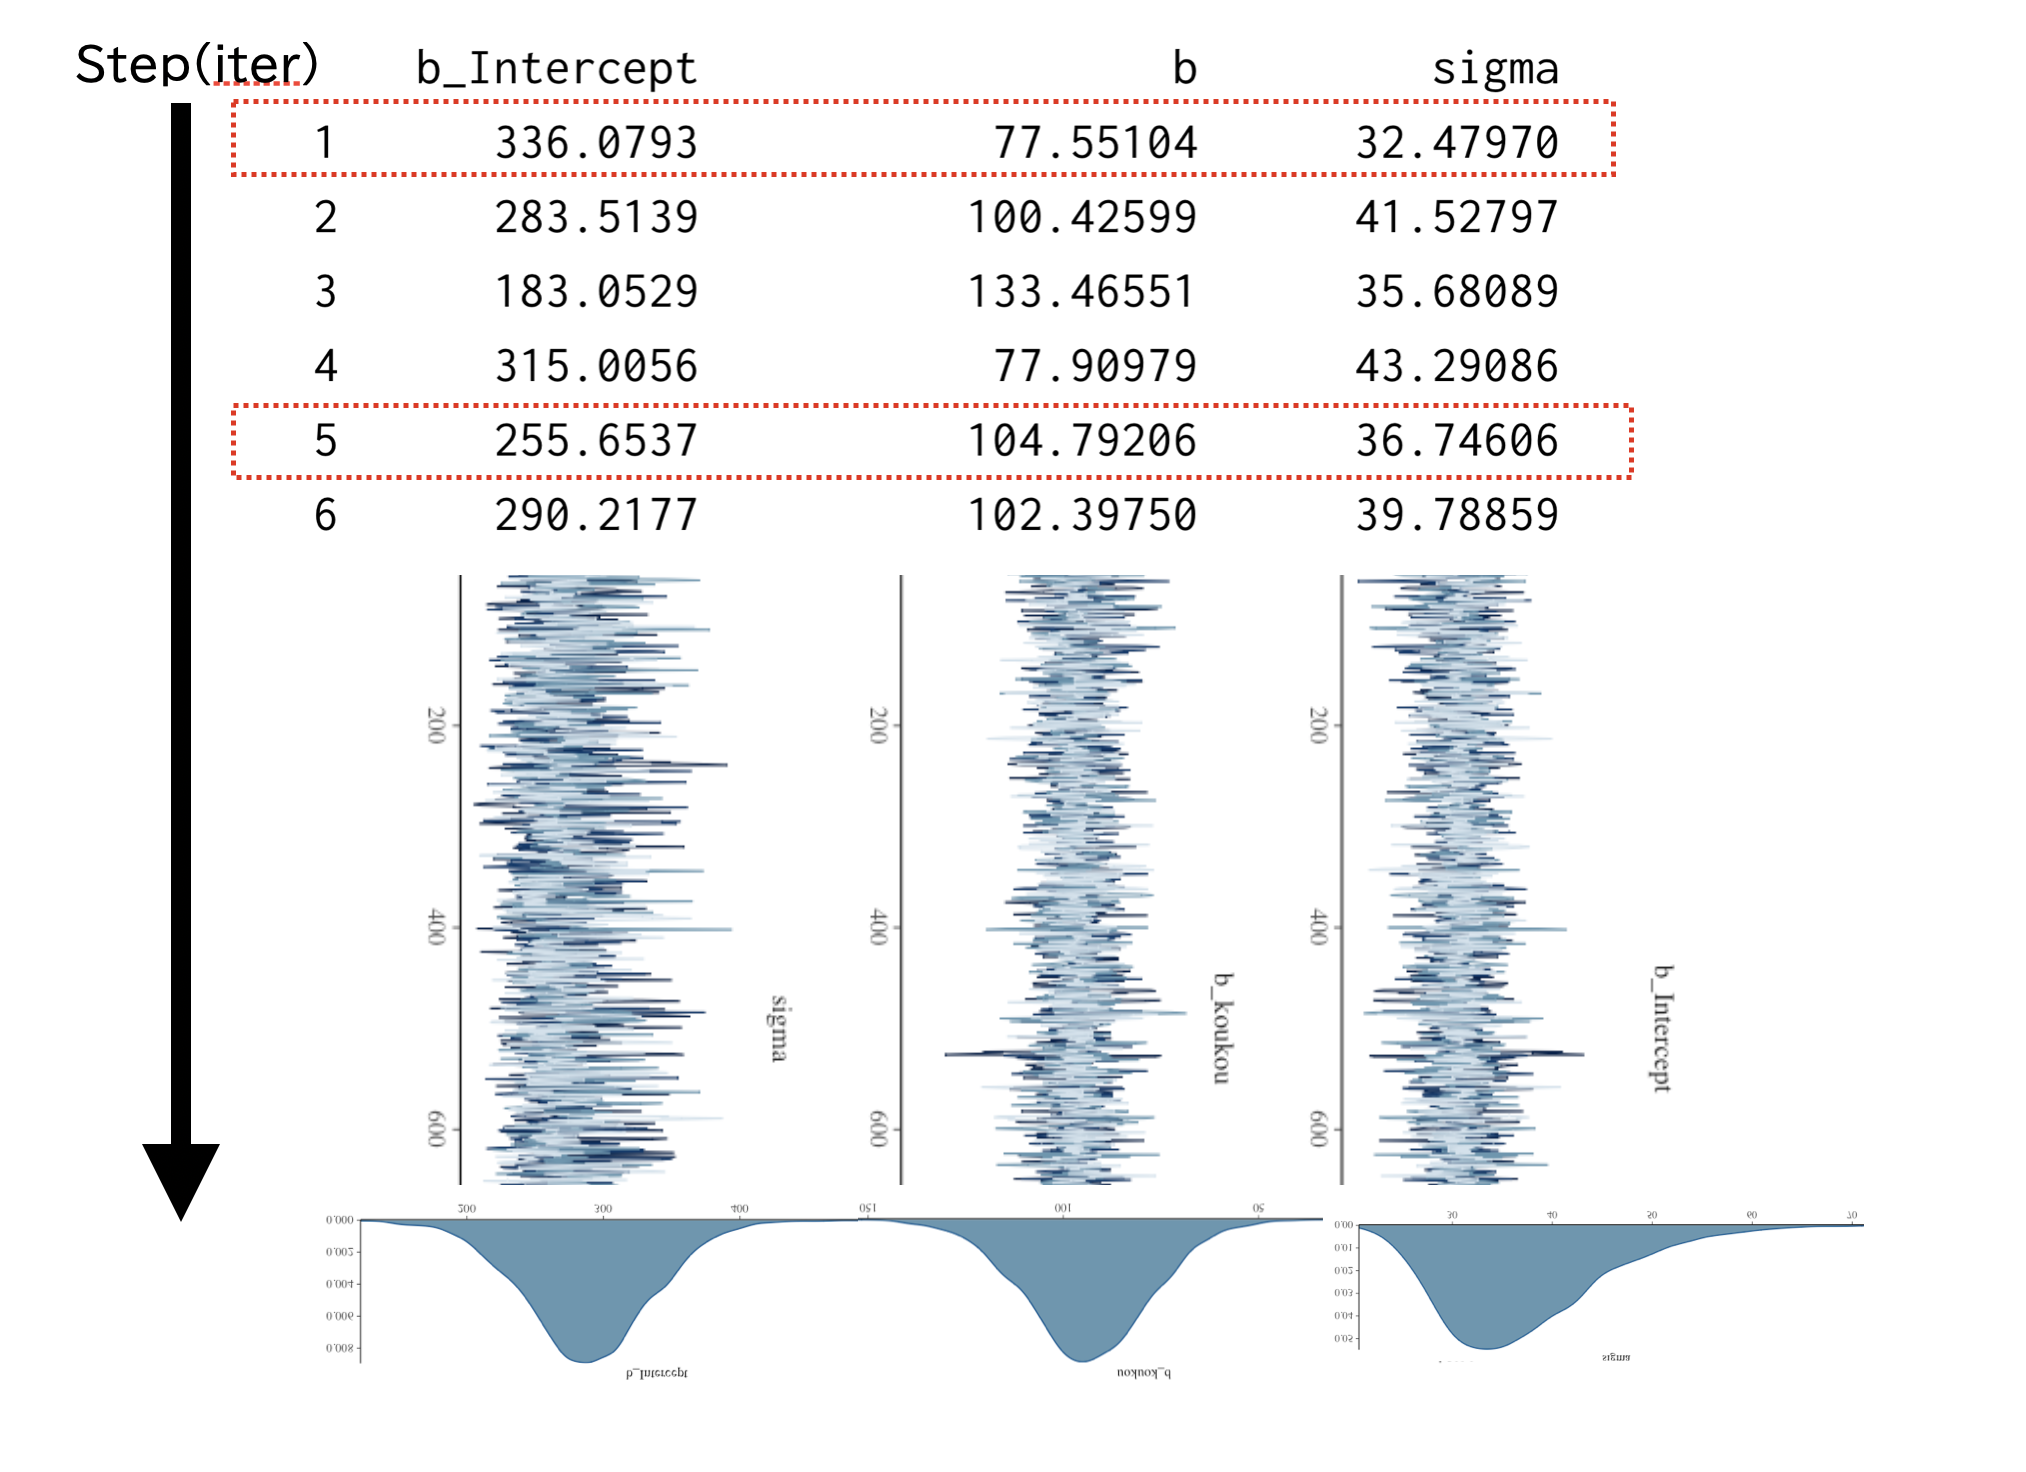
\includegraphics[keepaspectratio,width=0.8\linewidth]{../images/27_bayesian3/slide27_02.png}
   \caption{What MCMC is doing}
   \label{fig::27_02}
\end{figure}



% これを踏まえて，出力されたものを見てみましょう。まず\texttt{4 chains}とあります。これはMCMCのステップを4つ並行して実行したことを意味しています。MCMCはステップ・バイ・ステップで，一歩ずつ次の乱数を生み出していってるわけですが，どこからスタートするかによって全然違う答えにたどり着いてしまう可能性がゼロではありません。ステップの途中でも，もしかすると変なところにフラフラ外れていってしまっているかもしれません。こうした懸念をチェックするべく，1つのマルコフチェインではなくて複数のチェインを同時に実行して，「どのチェインも同じところに行き着くよ」ということを持って，正しくサンプリングがなされたと判断するのです。
Considering this, let's look at the output. First, there are \texttt{4 chains}. This means that the steps of the MCMC were executed in parallel four times. MCMC proceeds step by step, generating random numbers one at a time, but there is a non-zero chance that depending on where you start, it may lead to completely different answers. Even in the middle of the steps, it might be wandering off to weird places. To check against such concerns, we run multiple chains at once rather than a single Markov chain, and judge that sampling has been done correctly when "all chains end up in the same place".

% 次に\texttt{iter}とあります。これは総ステップ数で，今回は各チェイン2000ステップしたことを意味します。次に\texttt{warmup}は，ウォームアップ期間とかバーンイン期間と呼ばれるものです。チェインの最初の方のステップは，初期値に依存したステップになっており，事後分布の代表値としては適切でないかもしれません。事後分布をうまく代表するように，最初の期間は採用しないという方法が取られており，それが最初の1000ステップであること記録されています。各チェインについて2000ステップ，うち1000ステップを捨てるので1000ステップだけ採用されますが，それが4チェインあるので，合計で4000サンプル。4000点のヒストグラムで事後分布を描画したことになります。\texttt{ total post-warmup samples = 4000}というのはそういう意味ですね。最後に\texttt{thin=1}とありますが，これは間引きといわれ，サンプルとして採用するステップの間隔を意味します。今回は1ですので毎回のサンプルを(1stepずつ)採用していきますが，これが2とか3になると，2ステップ，3ステップごとにしか結果として保存しないということになります。
Next, there is \texttt{iter}. This refers to the total number of steps, which in this case means that each chain has taken 2000 steps. Next, \texttt{warmup} is what is called the warm-up period or burn-in period. The steps in the beginning of the chain may be steps dependent on the initial values, which may not be suitable as representative values of the posterior distribution. In order to well represent the posterior distribution, a method is taken where the initial period is not adopted, and it is recorded that it is the first 1000 steps. Each chain takes 2000 steps, discards 1000 steps, and only adopts 1000 steps, but since there are 4 chains, there are a total of 4000 samples. A histogram of 4000 points was used to draw the posterior distribution. \texttt{total post-warmup samples = 4000} means that. Finally, there is \texttt{thin=1}, which refers to thinning, or the interval of steps adopted as samples. This time it is 1, so every sample will be adopted (1 step at a time), but if this becomes 2 or 3, results will only be saved every 2 steps, 3 steps, and so on.

% 図\ref{fig::27_03}をみてください。この図はトレースプロットといい，先ほどの図\ref{fig::27_02}の中頃にあったもの，あるいは\texttt{plot}で出力させた図\ref{fig::27_01}の右側にあったものです。ステップ数を横軸にとりながら鎖のステップを線で結んで，鎖がどのあたりをウロウロしているかを可視化しています。図の上には，複数のスタート地点から始まっても，途中で鎖が絡まりあって同じような領域をウロウロしている(サンプリングしている)ことが示されています。一方，下の方の図では鎖がほぐれています。下のような例は，サンプリングがうまくいっていないことの証左で，モデルが悪かったか，パラメータを特定する条件が不十分であったか，といった何らかの問題があったことを示しています。
Please refer to Figure \ref{fig::27_03}. This chart is known as a trace plot and is the one that was in the middle of the previous figure \ref{fig::27_02}, or was on the right side of the figure \ref{fig::27_01} outputted by \texttt{plot}. It visualizes where the chain is roving by drawing the steps of the chain while taking the number of steps as the horizontal axis. The top of the diagram shows that even if it starts from multiple starting points, the chains are tangled midway, roving (sampling) within similar regions. On the other hand, the chains are unraveled in the lower diagram. Instances like those in the bottom are evidence that the sampling has not been successful and indicate that there was some problem, such as a bad model or insufficient conditions for specifying parameters.
\begin{figure}[ht]
   \centering
   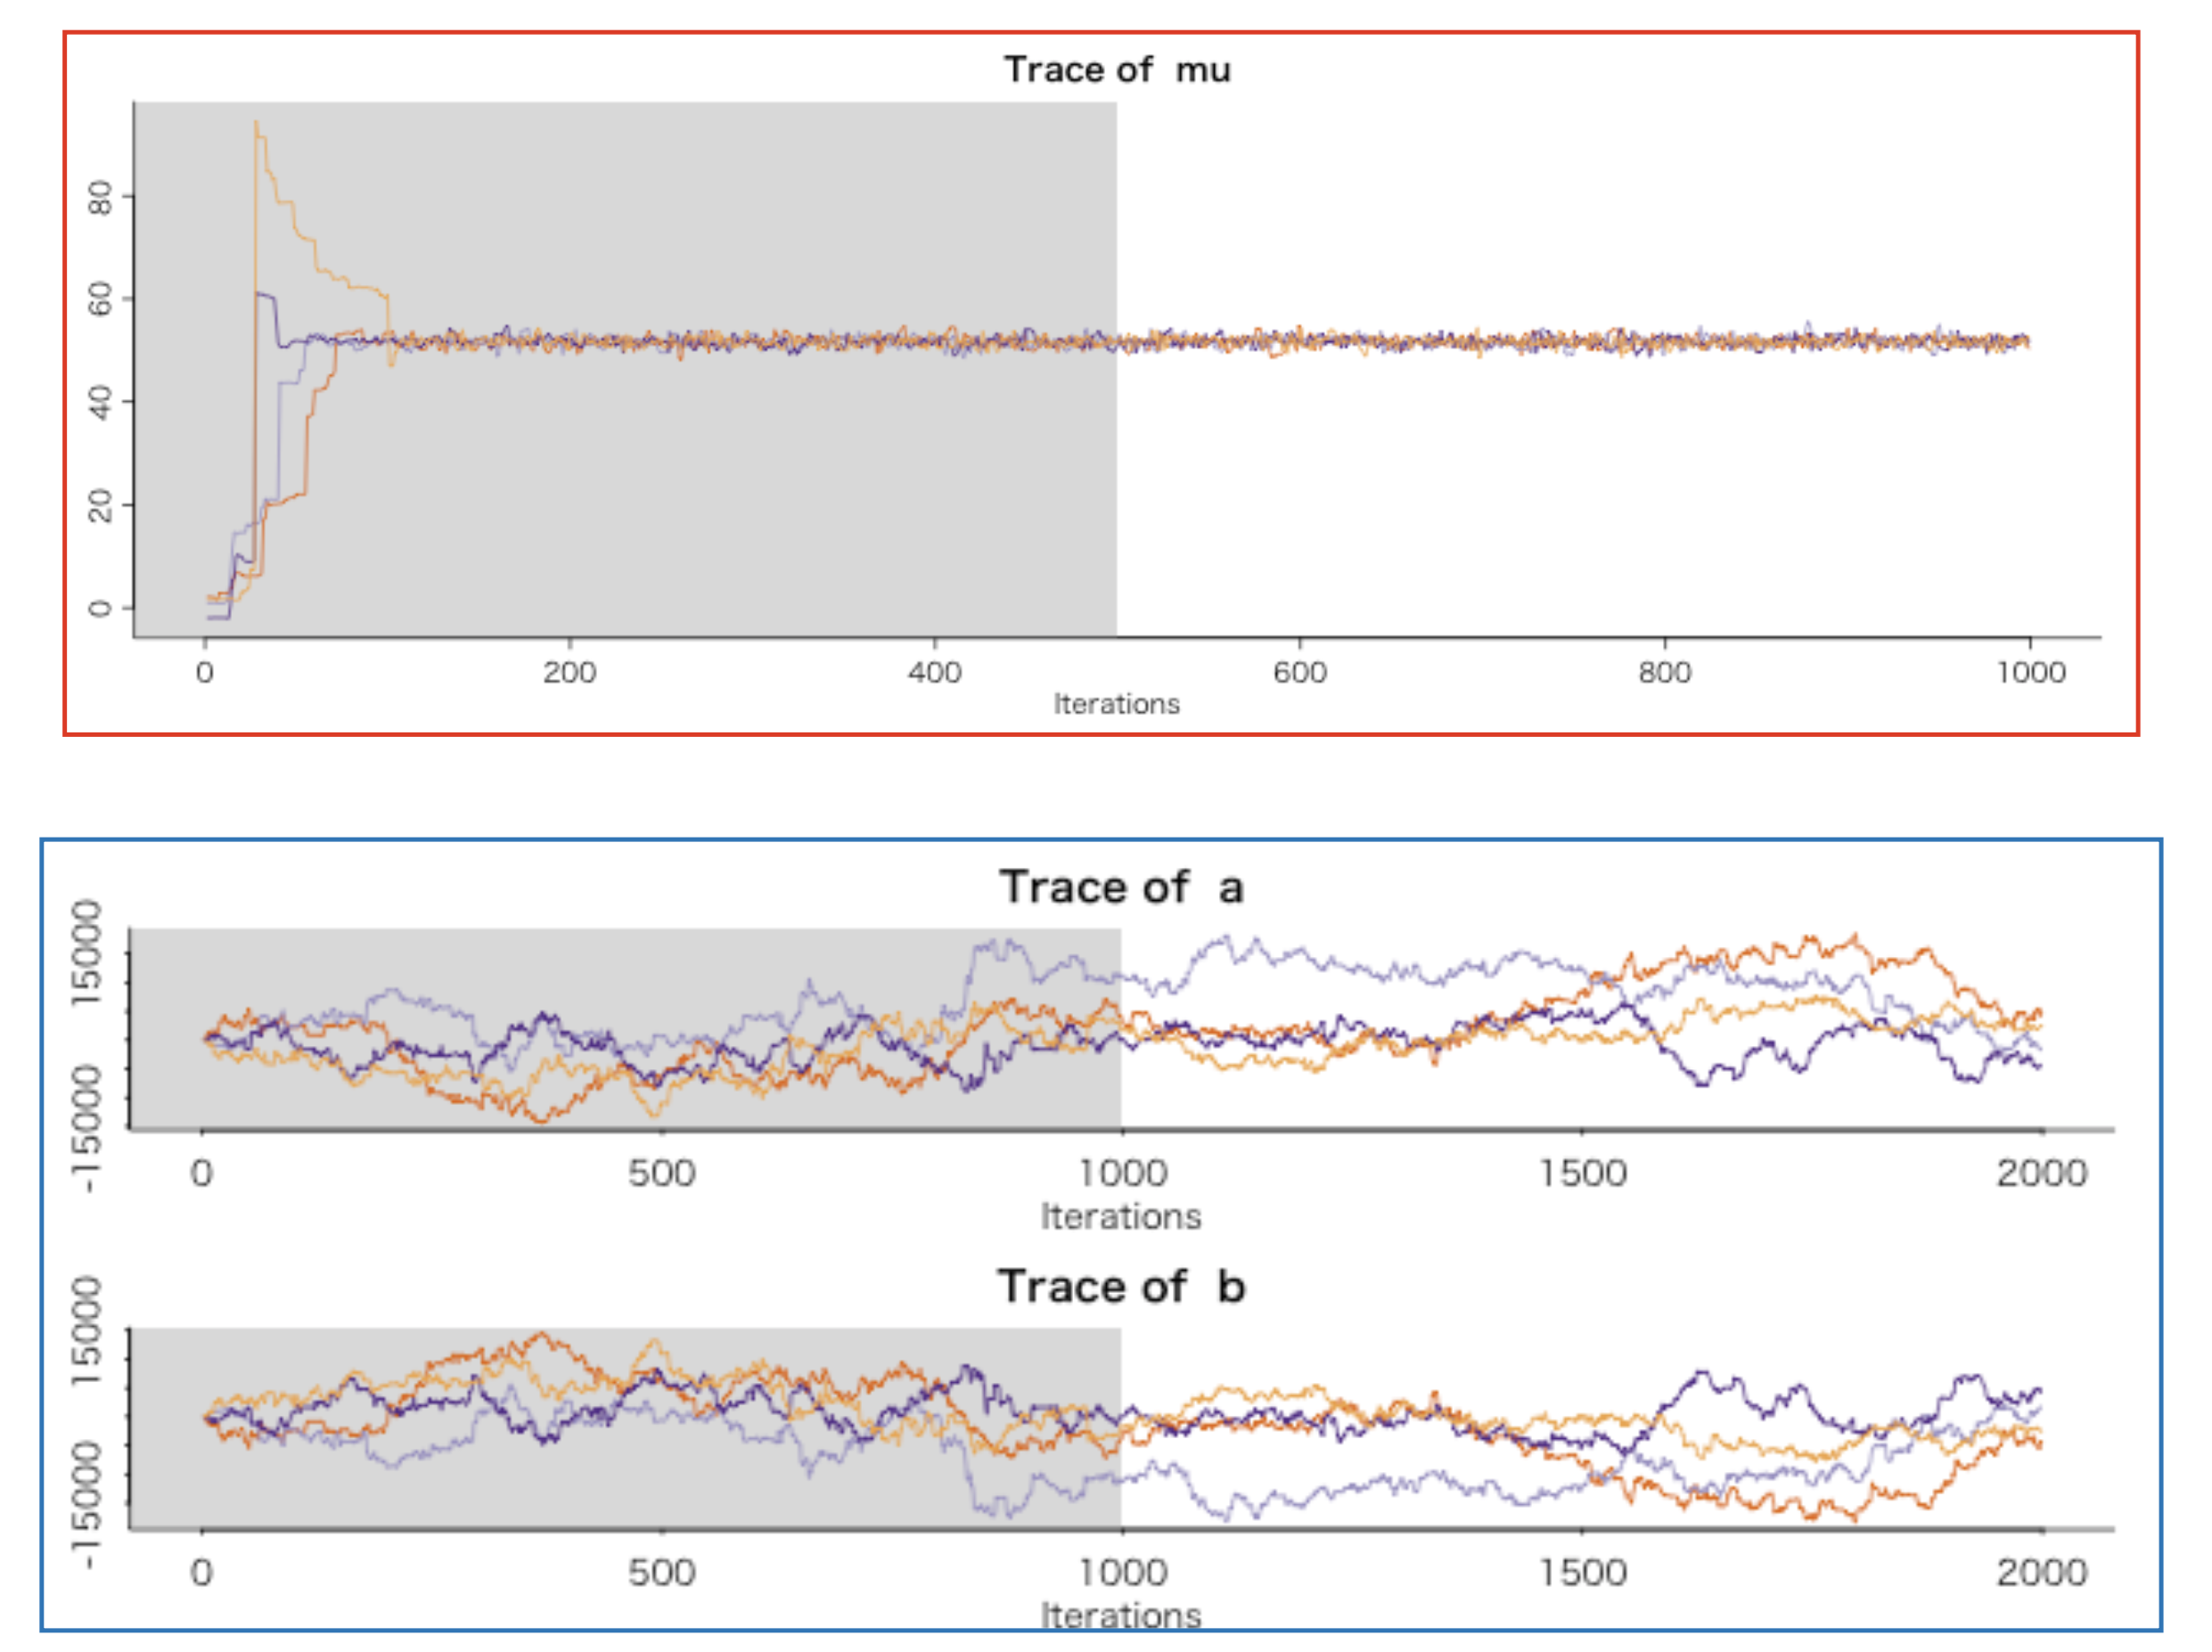
\includegraphics[keepaspectratio,width=0.8\linewidth]{../images/27_bayesian3/slide27_01.png}
   \caption{Example of estimation failure}
   \label{fig::27_03}
\end{figure}

% このように，結果が出力された後でMCMCの挙動をチェックすることが必要です。出力画面には最後にチェインの絡み具合をし評価した$\hat{R}$(Rhat)が1であれば収束している，ということを書いていて\footnote{ひとところに集まってきているという意味のconvergeを収束，といいます。コロナウイルスの蔓延が終わる，という意味でのしゅうそくは「終息」と書きます。}，今回の結果のRhatの列にはいずれも1.00とありますから，MCMCは問題なく事後分布からの代表値を取り出している，と診断できます(\texttt{Rの出力\ref{RS:out27_04}})。
In this way, it is necessary to check the behavior of MCMC after the results are output. The output screen states at the end that if the $\hat{R}$(Rhat), which evaluates how the chains are entangled, is 1, it is considered to be converging\footnote{The term "converge," meaning coming together in one place, is translated as "converge." The end of the spread of the coronavirus is written as "end" in the context of "converging."}. As all the Rhat in the results of this time are written as 1.00, it can be diagnosed that MCMC is properly extracting representative values from the posterior distribution (R-output\ref{RS:out27_04}).

\begin{Rscreen}{Message about MCMC}{out27_04}
   \begin{verbatim}
and Rhat is the potential scale reduction factor on split 
chains (at convergence, Rhat = 1).
\end{verbatim}
\end{Rscreen} 

English translation:
The message pertains to MCMC. The term "Rhat" refers to the potential scale reduction factor on split chains. At the point of convergence, Rhat equals 1.


% \section{要因計画の推定}
\section{Estimation of Factorial Design}
% 続いて要因計画の例にいきましょう。既に線形モデルで推定する方法については説明してありますから，これの関数を\texttt{lm}から\texttt{brm}に変えるだけでオッケーです。二要因の例を使って説明してみましょう(\texttt{code:\ref{code:27_06}})。
Let's move on to an example of factorial design. Since the method of estimation in the linear model has already been explained, it's okay to simply change the function from \texttt{lm} to \texttt{brm}. Let's explain using an example of two factors (\texttt{code: \ref{code: 27_06}}).

\begin{lstlisting}[language=c++,label={code:27_06},caption={データを作ってbrmでベイズ推定}]
Example2 <- data.frame(
    id = 1:12,
    num = rep(1:3, 4),
    temp = rep(1:2, each = 6),
    maker = rep(rep(1:2, each = 3), 2),
    value = c(13, 11, 12, 7, 6, 8, 9, 9, 9, 13, 11, 9)
)
Example2$temp <- factor(Example2$temp,
                        labels = c("Hot", "Cold")
)
Example2$maker <- factor(Example2$maker,
                         label = c("A", "B")
)

result.brm2 <- brm(value ~ temp * maker, data = Example2)
result.brm2
\end{lstlisting}

% \paragraph{コード解説}
\paragraph{Code Explanation}
\begin{description}
   \item[1-7行目] データフレーム形にデータを組み上げています
   \item[8-13行目] 説明変数の中で名義尺度水準のものを要因型であると設定しています。
   \item[15行目] 線形モデルを実行しています。\texttt{brm}としてあることに注意して下さい。
   \item[16行目] 結果を出力させています。
\end{description}

% これを実行した結果が次のようになります(\texttt{Rの出力\ref{RS:out27_05}})。
The result of executing this will be as follows (R output \ref{RS:out27_05}).
\begin{Rscreen}{交互作用モデルのbrms結果}{out27_05}
   \begin{verbatim}
Family: gaussian 
Links: mu = identity; sigma = identity 
Formula: value ~ temp * maker 
 Data: Example2 (Number of observations: 12) 
Samples: 4 chains, each with iter = 2000; warmup = 1000; thin = 1;
       total post-warmup samples = 4000

Population-Level Effects: 
              Estimate Est.Error l-95% CI u-95% CI Rhat Bulk_ESS Tail_ESS
Intercept          12.01      0.84    10.34    13.65 1.00     1742     2016
tempCold           -3.04      1.21    -5.55    -0.68 1.00     1554     1583
makerB             -5.02      1.19    -7.40    -2.63 1.00     1622     1915
tempCold:makerB     7.05      1.65     3.69    10.42 1.01     1475     1563

Family Specific Parameters: 
    Estimate Est.Error l-95% CI u-95% CI Rhat Bulk_ESS Tail_ESS
sigma     1.42      0.42     0.85     2.49 1.00     1290     1796

Samples were drawn using sampling(NUTS). For each parameter, Bulk_ESS
and Tail_ESS are effective sample size measures, and Rhat is the potential
scale reduction factor on split chains (at convergence, Rhat = 1).
\end{verbatim}
\end{Rscreen}

% データの生成に正規分布を仮定していること(\texttt{Family: gaussian})，モデル式やMCMCサンプルの特徴を描いた後に，推定値が出ています。推定値の見方は\texttt{lm}の時と同じですが，95\%区間が示されていること，MCMCの収束を判定する\texttt{Rhat}などがあるところが違うところですね。この95\%区間が狭いと自信を持って結果を言える，広いと確信度が低くまだまだデータが足りない，というところでしょうか。また今回は主効果にあたるところの95\%区間が0を跨いでいるので，傾きが0であるという帰無仮説を考えるのであれば，これは棄却できないということになります。交互作用は少なくとも3.69，大きければ10.42ポイントも動かすのですから，これは大きな効果があると言っていいでしょう。
It is assumed that the data is generated in a normal distribution (Family: gaussian). After describing the characteristics of the model formula and MCMC samples, the estimated values are presented. The way to read the estimated values is the same as when using \texttt{lm}, but there are differences such as the display of the 95% interval and the presence of \texttt{Rhat} for determining the convergence of MCMC. If the 95% interval is narrow, we can confidently state the results, while if it's wide, there's low confidence and it would suggest that more data is needed. In this case, the 95% interval for the main effect crosses 0. Thus, if we consider the null hypothesis that the slope is zero, we cannot reject it. The interaction effect moves at least 3.69 points, and possibly up to 10.42 points, so we can say that this has a significant effect.

% このように直接的に大きさを評価することもできますが，次のようなプロットを描くととくにわかりやすいでしょう(\texttt{code:\ref{code:27_07}})。
You can also evaluate the size directly like this, but it might be particularly easy to understand if you draw a plot as follows (code:\ref{code:27_07}).
Sorry, it seems that the given TeX code is not in Japanese but rather in a programming language called C++. It shows a code snippet that calls a function called `conditional_effects` three times with different arguments to see the effects of conditioning on the result of a Bayesian regression model. The function is used to analyze the effects of two variables, "temp" and "maker", as well as their interaction ("temp:maker").

% 表示される3つの図(\ref{fig::27_04})はそれぞれ，温度の主効果，銘柄の主効果，そして交互作用であり，そのEAP推定値(点)と95\%確信区間がついています。これを見ると，温度の主効果は確信区間に重複があり，銘柄にそれはないこと，交互作用も暖かい時の銘柄の違いが大きく，冷たい時の銘柄の効果は薄いとか，銘柄Bは温度ではっきりと違いがあるというようなことが目に見えてわかります。これらは帰無仮説検定ではありませんから，検定の多重性の問題がないため，新しい統計量を使って計算し直す必要もありません。非常に直感的に推論を進めていくことができるでしょう。
The three figures shown (\ref{fig::27_04}) respectively represent the main effects of temperature, brand, and their interaction, along with their EAP estimates (dots) and 95% confidence intervals. Upon inspection, it's clear that while there is overlap in the confidence interval for the main effect of temperature, this is absent for the brand. The interaction also reveals notable differences between brands when it's warm, with a less pronounced effect observed when it's cold. For instance, brand B exhibits a distinct variance with temperature. These observations are not part of a null hypothesis test, therefore, there are no issues with multiple testing, and there is also no need to recalculate using a new statistic. Inference can proceed very intuitively.
\begin{figure}[ht]
   \centering
   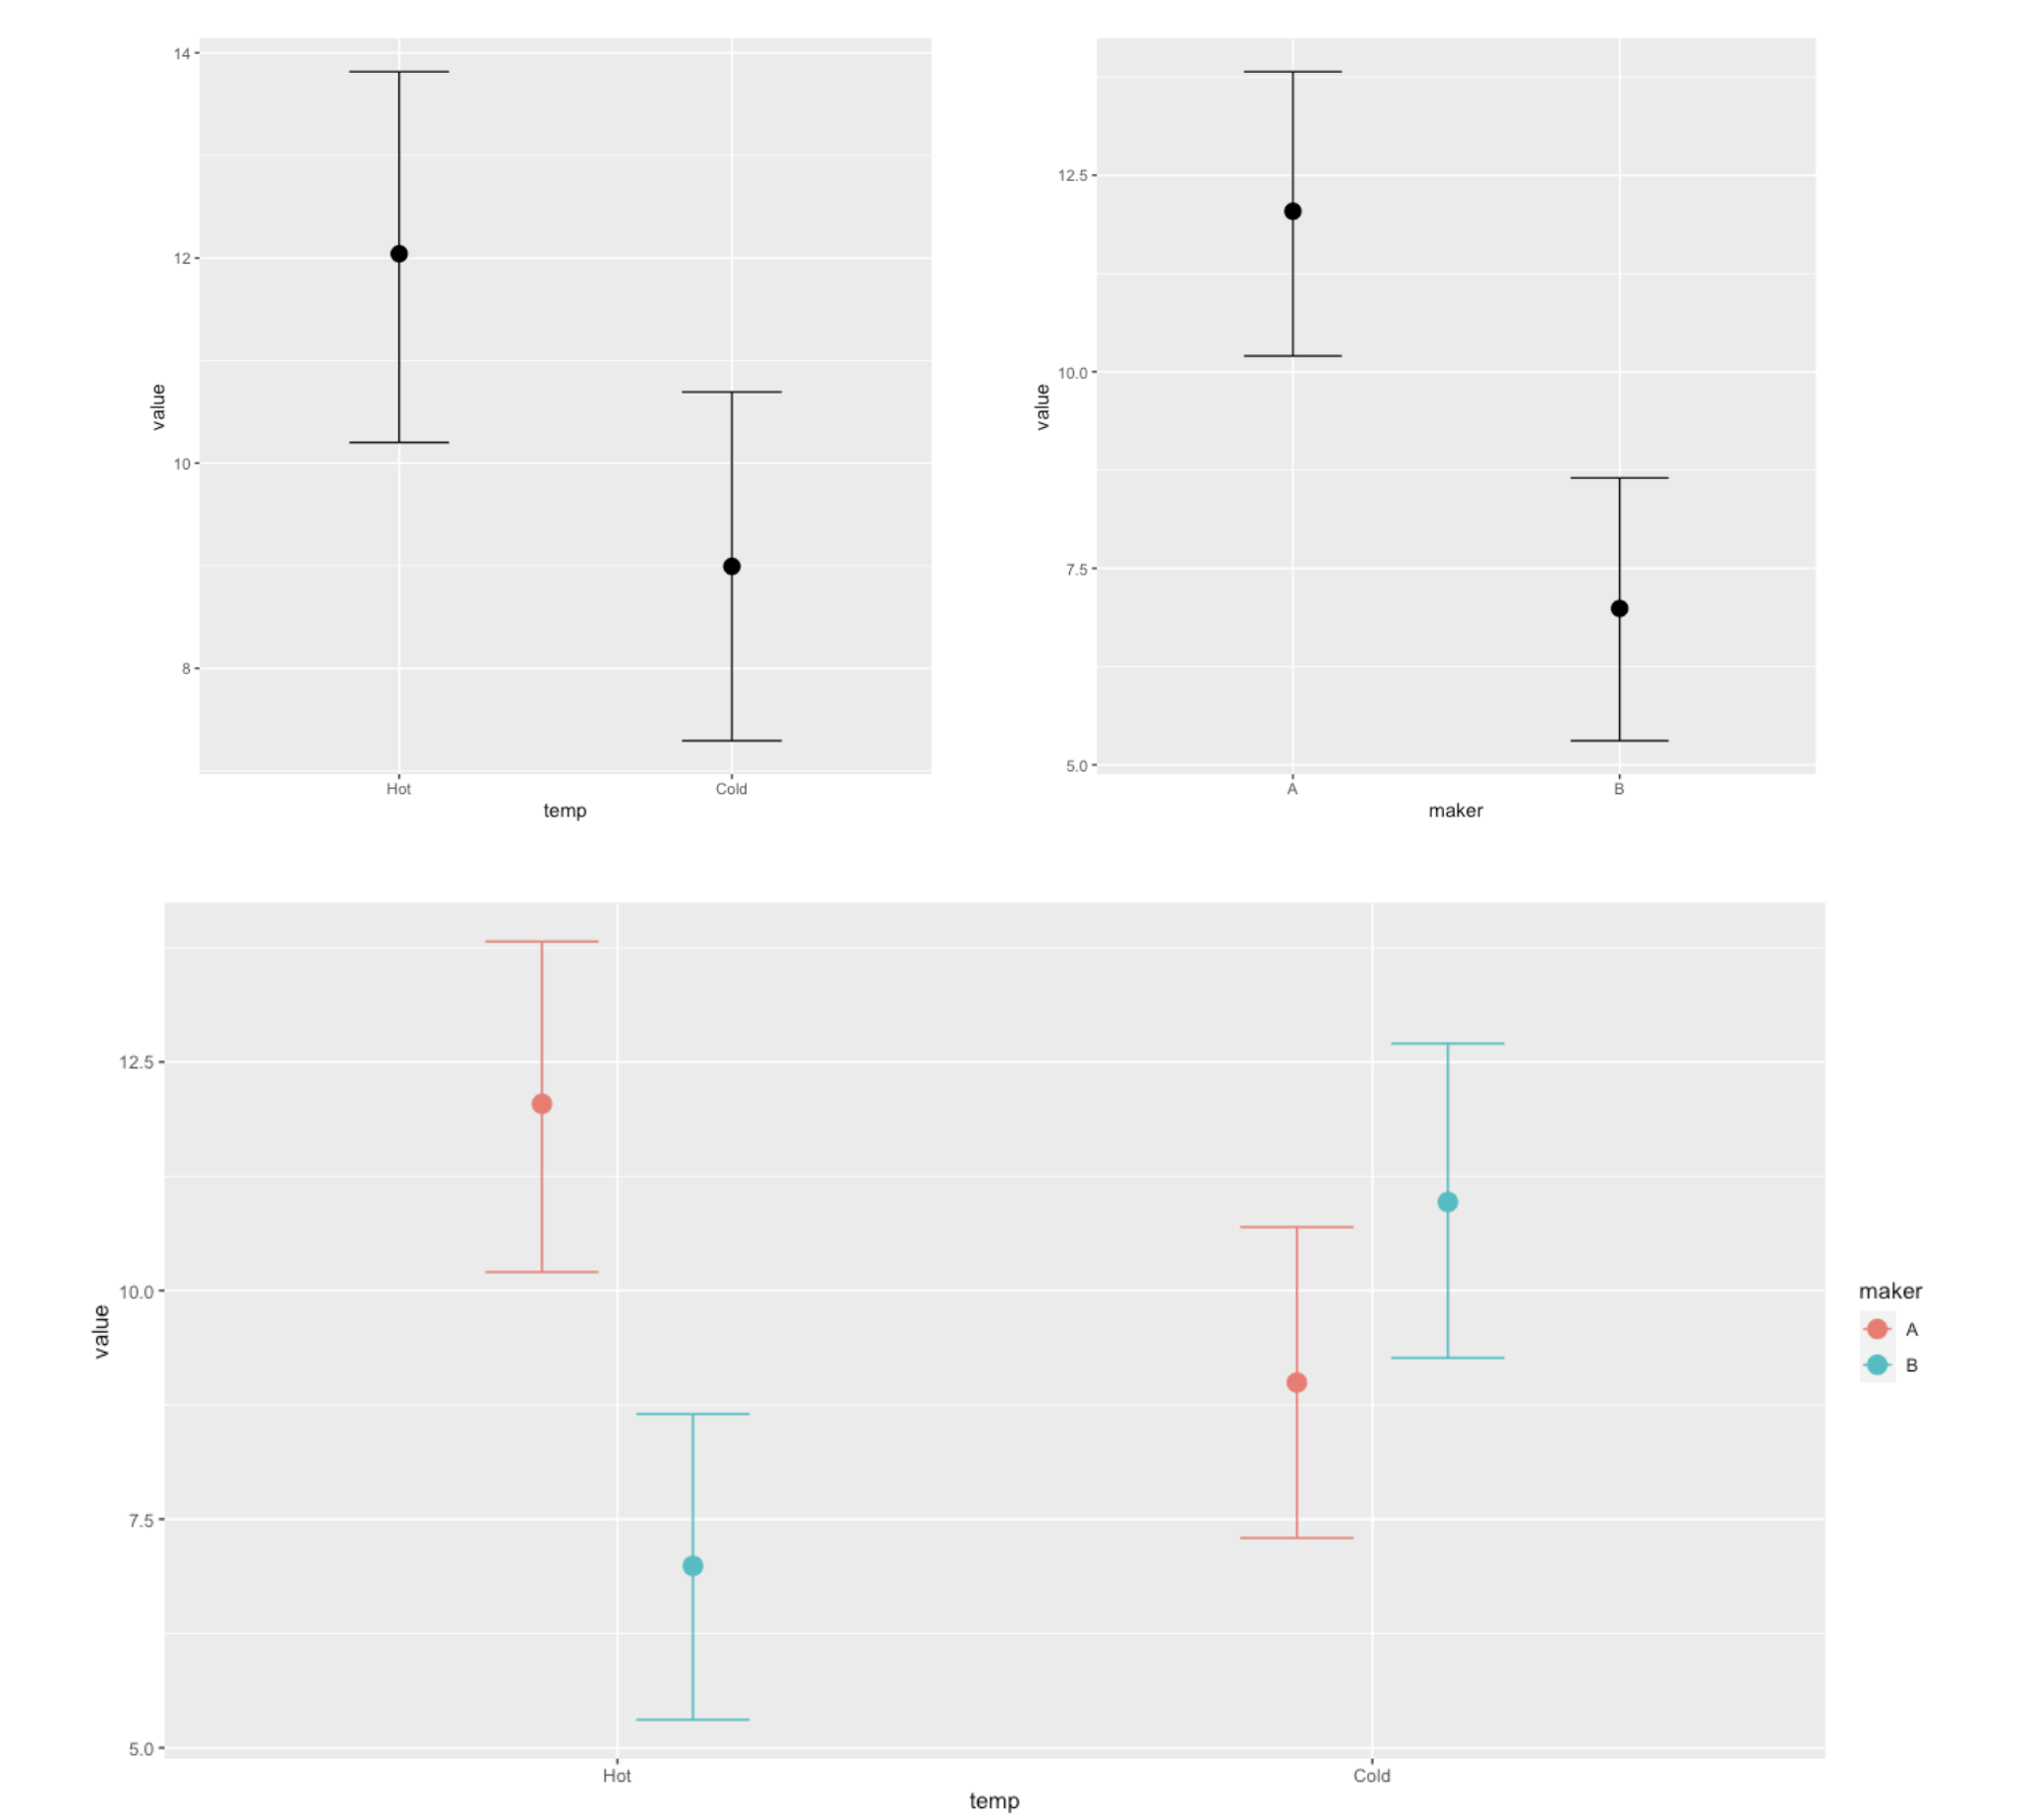
\includegraphics[keepaspectratio,width=0.8\linewidth]{../images/27_bayesian3/slide27_03.png}
   \caption{Estimation result of marginal mean value}
   \label{fig::27_04}
\end{figure}


% \section{群内モデルの推定}
\section{Estimation of In-group Model}
% 最後に，群内のモデルについて解説します。第\ref{m22_anovaOnR}講の，介入効果のモデルを思い出してください。群内要因がある線形モデルは，次のように表記できるのでした。
Finally, I will explain the model within the group. Recall the model of intervention effects from lecture \ref{m22_anovaOnR}. The linear model with a group factor could be denoted as follows.
\[ X_{ij} = \mu_i + \beta_0 + \beta_{ij} + \varepsilon_{ijk}\]
群間要因のモデルと違って，$\mu_i$すなわち個人$i$ごとの平均値が想定されていることがポイントです。これを確率モデルとして書くと，
\[ X_{ij} \sim Normal( \mu_i + \beta_0 + \beta_{ij} ,\sigma)\]
% となります。平均にあたるところが線形モデルで表現され，誤差$\varepsilon$が散らばることが正規分布の標準偏差$\sigma$で表現されていることを確認してください。それ以外に違いはありません。
This translates to: "Please confirm that the average is represented by the linear model and the error ε is represented by the standard deviation σ of the normal distribution. There is no other difference."
% ところで，個人差$i$は介入前のスタート地点の状態を表しており，さまざまな値を取ると考えられますが，この個性の部分についても正規分布を仮定できます。つまり，
By the way, the individual difference $i$ represents the state of the starting point before intervention, and is thought to take various values, but we can also assume a normal distribution for this individuality part. In other words,
\[ \mu_i \sim Normal(\mu_G, \tau) \]
のように，です(個人差の散らばりを表す標準偏差として，新たな記号$\tau$(タウ)を用意しました)。線形モデルで表現するには，このように正規分布の中に正規分布が入っている，という階層的な構造を考えることと同じなのです。これを\texttt{brms}で推定するには，次のようにコードを書きます(\texttt{code:\ref{code:27_08}})。
\begin{lstlisting}[language=c++,label={code:27_08},caption={データを作ってbrmでベイズ推定}]
Example3 <- data.frame(
  ID = rep(1:4,3),
  time = rep(1:3,each=4),
  value = c(10, 9, 4, 7,5, 4, 2, 3,9, 5, 3, 5)
)
Example3$time <- factor(Example3$time,labels = c("time1","time2","time3"))

result.brm3 <- brm(value ~ time + (1 | ID), data = Example3)
result.brm3
conditional_effects(result.brm3)
\end{lstlisting}
\paragraph{コード解説}
\begin{description}
	\item[1-5行目] データフレーム形にデータを組み上げています。前回と同じデータなのですが，組み方が少し変わっている点に注意してください。確認のために，\texttt{Example3}がどのような形になっているか一度表示してみるといいでしょう。
	\item[6行目] 説明変数の中で名義尺度水準のものを要因型であると設定しています。
	\item[8行目] 線形モデルを実行しています。\texttt{brm}としてあること，\texttt{(1|ID)}という項が増えていることに注意してください。
	\item[9-10行目] 結果を出力させています。
\end{description}
線形モデルの書き方が変わったことに注意してください。従属変数と独立変数をチルダで繋ぐのはこれまでと同じなのですが，これに加えて\texttt{(1|ID)}という表記があります。このカッコの中身は1が切片を表しており，それが変数\texttt{ID}ごとに変わるよ，ということを意味しています。

これを実行した結果が次のようになります(\texttt{Rの出力\ref{RS:out27_06}})。
\begin{Rscreen}{ランダム切片モデル}{out27_06}
	\begin{verbatim}
Family: gaussian 
Links: mu = identity; sigma = identity 
Formula: value ~ time + (1 | ID) 
 Data: Example3 (Number of observations: 12) 
Samples: 4 chains, each with iter = 2000; warmup = 1000; thin = 1;
       total post-warmup samples = 4000

Group-Level Effects: 
~ID (Number of levels: 4) 
            Estimate Est.Error l-95% CI u-95% CI Rhat Bulk_ESS Tail_ESS
sd(Intercept)     2.33      1.15     0.69     5.20 1.00      970     1001

Population-Level Effects: 
        Estimate Est.Error l-95% CI u-95% CI Rhat Bulk_ESS Tail_ESS
Intercept     7.36      1.30     4.79     9.83 1.00     1201     1112
timetime2    -3.99      1.00    -5.99    -1.86 1.00     2267     2017
timetime3    -2.00      0.98    -3.95    -0.02 1.00     2439     1736

Family Specific Parameters: 
    Estimate Est.Error l-95% CI u-95% CI Rhat Bulk_ESS Tail_ESS
sigma     1.31      0.51     0.70     2.58 1.01      957     1723

Samples were drawn using sampling(NUTS). For each parameter, Bulk_ESS
and Tail_ESS are effective sample size measures, and Rhat is the potential
scale reduction factor on split chains (at convergence, Rhat = 1).
\end{verbatim}
\end{Rscreen}
結果のところに大きく分けて，\texttt{Group-Level Effects}と\texttt{Population-Level Effects}の2つがあることみてください。群間要因の場合は\texttt{Population-Level Effects}の要素しかありませんでした。これは\keyterm{固定効果}{こていこうか}{fixed effect}と呼ばれ，どの個人にも共通の効果があることを表しています。これに対して\texttt{Group-Level Effects}は\keyterm{変量効果}{へんりょうこうか}{random effect}と呼ばれ，人ごと，ケースごとに確率的に変わりうるところを意味しています。今回は最初の個人差(スタート地点，切片)が人ごとに変わるので\texttt{sd(Intercept)}とあります。スタート地点が人によって2点ぐらいは左右するよ，ということがここでみて取れるのです。

固定効果の見方は，群間要因の時と同じです。第一期(Time1)に比べて，第二期は平均点が$-3.99$，第三期は$-2.00$となっています。この区間幅をみると，第一期よりも下がっているというところですが，第一期と第三期の下り幅はギリギリ0でない，というぐらいであってもう少し慎重にデータを追加して検証した方が良いかもしれませんね。\\

\section{課題}
第\ref{m22_anovaOnR}講でやった3つの課題それぞれを，\texttt{brms}パッケージを使って実行してください。念の為，以下に簡単な問題設定を再掲いたします。
\paragraph{課題1 線形モデルとしての分析}
ある学校の国語の授業で，ある教師が4つのクラスそれぞれに対して個別のテキストを使って授業を行い，同一のテストを行うことでテキストの効果があるかどうかを検証したとします。
各クラスには10人の生徒がいて，それぞれのテスト結果は表\ref{L23::exe1}の通りです。このデータについて，回帰分析のベイズ推定を行った上で，次の各問いに答えてください。

\begin{enumerate}
	\item 切片の推定値はいくらになりましたか。おおよそで結構ですので，EAP推定値を答えてください。
	\item 回帰分析を行った結果，テキストAにくらべてテキストBの平均値はどれぐらい違うと思われますか。おおよそで結構ですので，95\%区間を答えてください。
	\item 回帰分析を行った結果，テキストAにくらべてテキストCの平均値はどれぐらい違うと思われますか。おおよそで結構ですので，95\%区間を答えてください。
	\item 回帰分析を行った結果，テキストAにくらべてテキストDの平均値に違いがあると断言しても良いでしょうか。\verb|conditional_effects|の図をみて判断してください。
\end{enumerate}


\paragraph{課題2 Betweenデザインの分散分析}
別の学校では，テキストをA,B,Cの3種類とし，教員が二人がそれぞれのテキストを使って教えることにしました。1クラス12人，一学年6クラスを使っての実験です。
授業後のテストの点数が表\ref{L23::exe2}の通りです。このデータに対して回帰分析のベイズ推定を行った上で，その結果について回答してください。

\begin{enumerate}
	\item 切片の推定値はいくらになりましたか。おおよそで結構ですので，EAP推定値を答えてください。
	\item テキストA,B,Cの効果はどのように判断すれば良いでしょうか。\verb|conditional_effects|の図をみて考察してください。
	\item 教員A,Bの効果ははどのように判断すれば良いでしょうか。\verb|conditional_effects|の図をみて考察してください。
	\item 交互作用として，どのような特徴があるでしょうか。\verb|conditional_effects|の図をみて考察してください。
\end{enumerate}

\paragraph{課題3 Withinデザインの分散分析}
さらに別の学校では，テキスト・教員は一種類・一人なのですが，4つの時期において成績が変化するかどうかを追跡調査しました。
各時期のテストの点数は表\ref{L23::exe3}の通りです。次の各指示に従い，その結果について回答してください。

なお，このデータセットは\texttt{Lesson8exe3.csv}ファイルに入っていますが，分析に際しては次のコードを実行して，整理しなおしたデータセットを使ってください(\texttt{code:\ref{code:27_09}})。
\begin{lstlisting}[language=c++,label={code:27_09},caption={データを外部ファイルから読み込んで実行する}]
library(tidyverse)
dat3 <- read_csv("Lesson8exe3.csv") %>% 
    pivot_longer(-id,names_to="period") %>% 
    print
\end{lstlisting}
\paragraph{コード解説}
\begin{description}
	\item[1行目] データファイル\texttt{Lesson8exe3.csv}を読み込んでいます
	\item[2行目] id列をキーにデータを縦型にしています
	\item[3行目] データを表示させています
\end{description}
\begin{enumerate}
	\item 個人差について正しく述べている文章を選んでください。
	\item 時期の効果について正しく述べている文章を選んでください。
\end{enumerate}

\end{document}
